\section{Results}
\label{sec:results}

We first ask how forecastable delayed onsets are and which observers capture the signal (\secref{sec:rq1}, \secref{sec:ew}). We then test whether an explicit forecast representation beats a matched direct reader (\secref{sec:rq2}). Finally we report activation history, question generalization, the story setting, and detection (\secref{sec:extra}).

\begin{figure}[t]
\centering
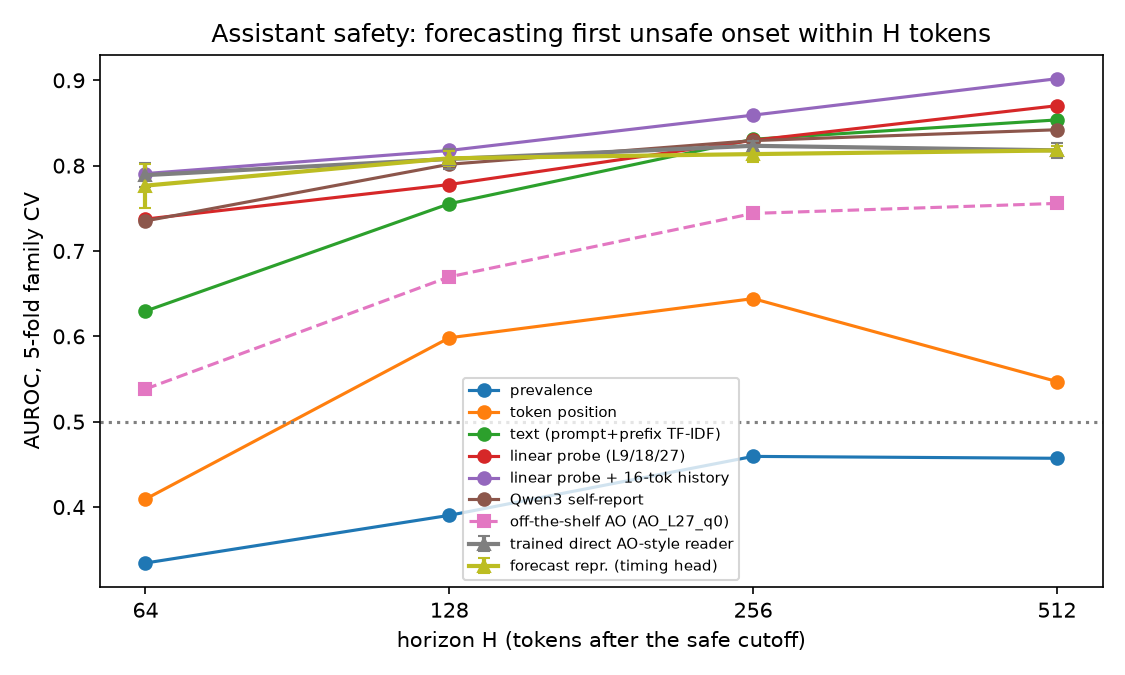
\includegraphics[width=0.85\linewidth]{figures/forecast_auroc_by_horizon_all.png}
\caption{{\bf \auroc by horizon} for the assistant setting (5-fold family CV). No informative method decays with lead distance; every method is weakest at $H{=}64$, where few positives exist and they must be separated from earlier prefixes of the same trajectory. \histprobe (purple) is best at every horizon. The off-the-shelf \ao (pink, dashed) is near chance at $H{=}64$. The \direct (gray) and \forecast (olive) readers nearly overlap and flatten at about 0.82.}
\label{fig:auroc}
\end{figure}

\begin{table}[t]
\centering
\caption{{\bf Forecasting the first unsafe onset within $H$ tokens} (assistant setting, safe prefixes only, 5-fold family CV, $n{=}3{,}520$ prefixes from 880 families). Cells give \auroc with 95\% family-bootstrap CIs. Trained readers give mean$\pm$sd over 3 seeds. \auprc and Brier are at $H{=}512$ (prevalence 10.7\%). Best in {\bf bold}. $^*$Out-of-fold constant predictions; values below 0.5 are a fold-composition artifact, not a signal.}
\label{tab:main}
\resizebox{\textwidth}{!}{%
\begin{tabular}{@{}llcccccc@{}}
\toprule
& & \multicolumn{4}{c}{\auroc at horizon $H$} & \multicolumn{2}{c}{$H{=}512$} \\
\cmidrule(lr){3-6} \cmidrule(lr){7-8}
& \textsc{Method} & $64$ & $128$ & $256$ & $512$ & \auprc$\uparrow$ & Brier$\downarrow$ \\
\midrule
\multirow{4}{*}{\rotatebox{90}{\scriptsize Baselines}}
& Prevalence$^*$ & 0.33 & 0.39 & 0.46 & 0.46 & 0.10 & 0.096 \\
& Token position & 0.41 {\scriptsize[.27,.56]} & 0.60 {\scriptsize[.49,.72]} & 0.64 {\scriptsize[.58,.70]} & 0.55 {\scriptsize[.52,.57]} & 0.12 & 0.095 \\
& \textprompt (prompt only) & 0.69 {\scriptsize[.55,.80]} & 0.72 {\scriptsize[.65,.79]} & 0.76 {\scriptsize[.70,.81]} & 0.77 {\scriptsize[.72,.81]} & 0.28 & 0.087 \\
& \textprefix (prompt+prefix) & 0.63 {\scriptsize[.47,.77]} & 0.76 {\scriptsize[.67,.84]} & 0.83 {\scriptsize[.78,.88]} & 0.85 {\scriptsize[.82,.89]} & 0.45 & 0.080 \\
\midrule
\multirow{4}{*}{\rotatebox{90}{\scriptsize Probes}}
& Linear probe L18 & 0.71 {\scriptsize[.60,.80]} & 0.78 {\scriptsize[.71,.85]} & 0.82 {\scriptsize[.78,.86]} & 0.87 {\scriptsize[.85,.89]} & 0.44 & 0.075 \\
& Linear probe L9+18+27 & 0.74 {\scriptsize[.63,.83]} & 0.78 {\scriptsize[.71,.85]} & 0.83 {\scriptsize[.79,.87]} & 0.87 {\scriptsize[.85,.89]} & 0.46 & 0.075 \\
& MLP probe L9+18+27 & 0.72 {\scriptsize[.62,.81]} & 0.76 {\scriptsize[.69,.83]} & 0.80 {\scriptsize[.76,.83]} & 0.84 {\scriptsize[.81,.87]} & 0.39 & 0.104 \\
& \histprobe (L18 + 16-token mean) & {\bf 0.79} {\scriptsize[.71,.87]} & {\bf 0.82} {\scriptsize[.75,.89]} & {\bf 0.86} {\scriptsize[.82,.90]} & {\bf 0.90} {\scriptsize[.88,.92]} & {\bf 0.50} & {\bf 0.071} \\
\midrule
\multirow{3}{*}{\rotatebox{90}{\scriptsize Verbal.}}
& \selfreport (\qwen) & 0.74 {\scriptsize[.66,.82]} & 0.80 {\scriptsize[.75,.85]} & 0.83 {\scriptsize[.79,.87]} & 0.84 {\scriptsize[.80,.88]} & 0.39 & 0.080 \\
& \ao, best (L27, q0) & 0.54 {\scriptsize[.44,.65]} & 0.67 {\scriptsize[.59,.75]} & 0.74 {\scriptsize[.70,.79]} & 0.76 {\scriptsize[.72,.79]} & -- & -- \\
& \ao (L18, q0) & 0.50 {\scriptsize[.39,.61]} & 0.63 {\scriptsize[.56,.70]} & 0.71 {\scriptsize[.67,.76]} & 0.75 {\scriptsize[.72,.78]} & -- & -- \\
\midrule
\multirow{2}{*}{\rotatebox{90}{\scriptsize Trained}}
& \direct reader (QA) & {\bf 0.79}{\scriptsize$\pm$.01} & 0.81{\scriptsize$\pm$.01} & 0.82{\scriptsize$\pm$.01} & 0.82{\scriptsize$\pm$.01} & 0.40 & 0.105 \\
& \forecast reader (timing head) & 0.78{\scriptsize$\pm$.02} & 0.81{\scriptsize$\pm$.01} & 0.81{\scriptsize$\pm$.01} & 0.82{\scriptsize$\pm$.01} & 0.37 & 0.108 \\
\bottomrule
\end{tabular}}
\end{table}


\subsection{How forecastable are delayed onsets?}
\label{sec:rq1}

\para{Activations forecast delayed onsets moderately well.}
\Tabref{tab:main} and \figref{fig:auroc} show the main results. A linear probe on all three layers reaches \auroc 0.74 at $H{=}64$ and 0.87 at $H{=}512$. \histprobe, which adds the mean of the last 16 layer-18 activations, is the best method at every horizon: 0.79, 0.82, 0.86, and 0.90. It also has the best \auprc (0.50 at 10.7\% prevalence) and the best Brier score (0.071).

\para{The hardest target is imminent onset, not distant onset.}
We expected \auroc to decay as the event moves further away. We find the opposite: every informative method has its \emph{lowest} \auroc at $H{=}64$. \auroc at $H$ is not a pure lead-distance curve, because the positive set changes with $H$. At $H{=}64$ the positives are prefixes 0--63 tokens before onset. Their negatives include earlier prefixes of the \emph{same} harmful trajectories, which look very similar. At $H{=}512$, by contrast, almost every prefix of a harmful trajectory is positive, so the task becomes ``is this a harmful request that \qwen will comply with?''

\para{Much of the long-horizon signal is visible in text.}
The prompt alone gives \auroc 0.77 at $H{=}512$, and the prompt+prefix text model reaches 0.85. Activations add the most at short horizons and with history: at $H{=}64$, \histprobe scores 0.79 vs.\ 0.63 for \textprefix, while at $H{=}512$ the gap shrinks to 0.90 vs.\ 0.85. Because the benign source has no events, request-level detection inflates long-horizon \auroc for every method equally. \textprompt is therefore the right yardstick for that shortcut, and \histprobe beats it at every horizon.

\para{The off-the-shelf Activation Oracle is the weakest non-trivial method.}
Zero-shot, the \ao answers ``Yes'' to only 0.6--1.1\% of prefixes for q0 and 12--15\% for q1. Even after 1-D calibration of its logit margin, its best variant (layer 27, q0) scores 0.54 at $H{=}64$, with a CI that includes chance, and 0.76 at $H{=}512$. This is below every probe, text model, and self-report score at every horizon. Layer 27 (75\% depth) is the AO's best read layer, as in its training. \selfreport, which also verbalizes but uses the target itself, does much better (0.74 to 0.84). It ties single-position probes but stays below \histprobe.

\subsection{Early warning}
\label{sec:ew}

\begin{table}[t]
\centering
\caption{{\bf Early warning at a target 5\% benign false-alarm rate.} We score with the $H{=}512$ output and set the threshold on benign validation families inside each training fold. Columns give the fraction of unsafe test trajectories whose first alert comes at least $k$ tokens before onset, and the realized test FAR. 88 unsafe and 792 benign trajectories (\ao: 78 and 670, from its own validation carve-out). Trained readers average 3 seeds. Best in {\bf bold}.}
\label{tab:ew}
\begin{tabular}{@{}lcccc@{}}
\toprule
\textsc{Method} & $\ge 64$ & $\ge 128$ & $\ge 256$ & Test FAR \\
\midrule
Prevalence / token position & 0.00 & 0.00 & 0.00 & 0.00 \\
\textprompt & 0.17 & 0.17 & 0.12 & 0.06 \\
\textprefix & 0.42 & 0.42 & 0.34 & 0.05 \\
Linear probe L9+18+27 & 0.42 & 0.42 & 0.31 & 0.04 \\
MLP probe L9+18+27 & 0.39 & 0.39 & 0.24 & 0.03 \\
\histprobe & {\bf 0.57} & {\bf 0.56} & {\bf 0.43} & 0.06 \\
\selfreport & 0.39 & 0.38 & 0.30 & 0.06 \\
\ao (L27, q0; best \auroc) & 0.22 & 0.22 & 0.13 & 0.05 \\
\ao (L18, q0; best alerts) & 0.36 & 0.36 & 0.27 & 0.06 \\
\direct reader & 0.38 & 0.37 & 0.22 & 0.04 \\
\forecast reader & 0.37 & 0.36 & 0.20 & 0.04 \\
\bottomrule
\end{tabular}
\end{table}


\begin{figure}[t]
\centering
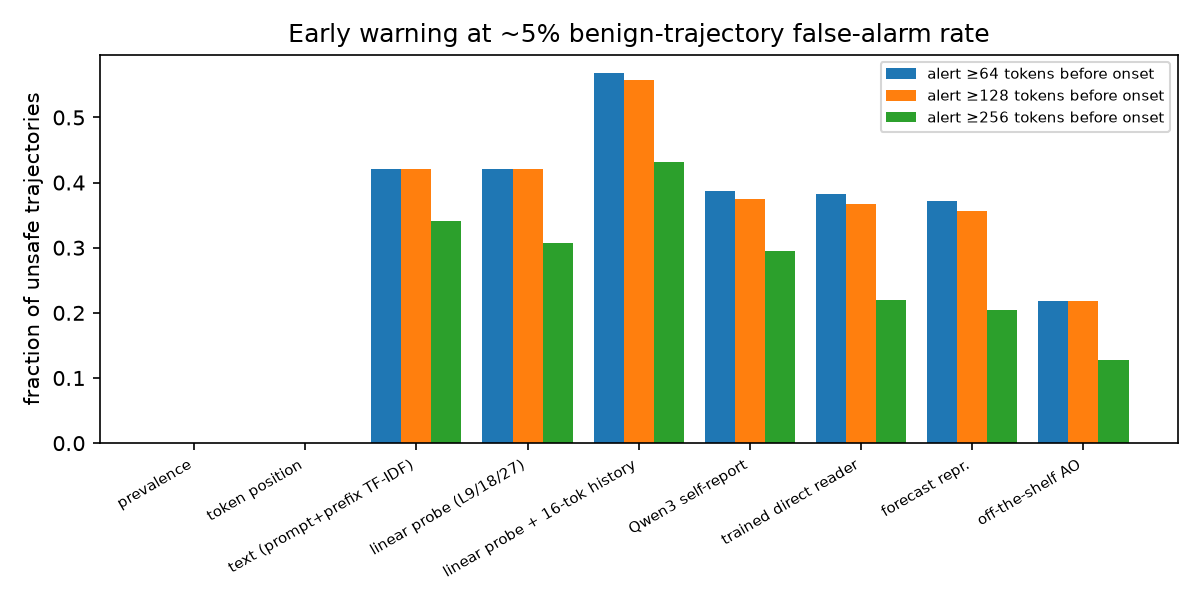
\includegraphics[width=0.85\linewidth]{figures/early_warning.png}
\caption{{\bf Early warning at about 5\% benign-trajectory false-alarm rate.} Bars show the fraction of unsafe trajectories alerted at least 64, 128, or 256 tokens before onset. \histprobe alerts on 56\% of trajectories at least 128 tokens ahead. The \ao bar shows the layer-27 q0 variant, which has the best \auroc but few alerts (22\%); the layer-18 q0 variant reaches 36\% (\tabref{tab:ew}).}
\label{fig:ew}
\end{figure}

\Tabref{tab:ew} and \figref{fig:ew} report the deployment-oriented metric. At a realized test FAR of 3--6\%, \histprobe alerts on 56\% of unsafe trajectories at least 128 tokens before onset. Single-position probes and \textprefix reach 42\%, \selfreport 38\%, and the trained readers 36--37\%. Prompt-only text reaches only 17\%, and prevalence and token position never alert. The $\ge$64 and $\ge$128 columns nearly coincide because onsets are late (median token 360) and alerts usually fire at the first cutoffs ($t{=}32$--$64$). When an alert happens, it is almost always far ahead; the main failure is \emph{missed} trajectories (40\% for \histprobe, 56\% for the linear probe). With 88 unsafe trajectories, the 95\% binomial interval around 0.37 is about $\pm$0.10, so the advantage of \histprobe over the trained readers (0.56 vs.\ 0.37) is about two standard errors.

\subsection{Does an explicit forecast representation help?}
\label{sec:rq2}

\begin{table}[t]
\centering
\caption{{\bf \forecast vs.\ matched \direct reader.} \auroc of seed-averaged out-of-fold predictions; $\Delta$ is the paired family-bootstrap difference with 95\% CI and two-sided $p$. Negative values favor \direct. Seed averaging (ensembling) gives higher \auroc than single seeds in \tabref{tab:main}.}
\label{tab:paired}
\resizebox{\textwidth}{!}{%
\begin{tabular}{@{}ccccll@{}}
\toprule
$H$ & \direct QA & \forecast head & \forecast QA & $\Delta$(head $-$ \direct) [CI], $p$ & $\Delta$(\forecast QA $-$ \direct) [CI], $p$ \\
\midrule
64  & {\bf 0.819} & 0.779 & 0.806 & $-0.040$ [$-0.093$, $0.005$], 0.10 & $-0.013$ [$-0.076$, $0.037$], 0.70 \\
128 & {\bf 0.844} & 0.826 & 0.811 & $-0.018$ [$-0.053$, $0.014$], 0.29 & $-0.034$ [$-0.081$, $0.010$], 0.13 \\
256 & {\bf 0.859} & 0.826 & 0.822 & $-0.033$ [$-0.056$, $-0.013$], 0.002 & $-0.038$ [$-0.062$, $-0.014$], $<$0.001 \\
512 & {\bf 0.851} & 0.833 & 0.821 & $-0.018$ [$-0.034$, $-0.003$], 0.014 & $-0.031$ [$-0.053$, $-0.011$], $<$0.001 \\
\bottomrule
\end{tabular}}
\end{table}


\para{The forecast representation does not beat the direct reader.}
\Tabref{tab:paired} compares seed-averaged out-of-fold predictions. The \forecast timing head trails \direct at every horizon: $\Delta$\auroc $=-0.040$, $-0.018$, $-0.033$, and $-0.018$ for $H=64$ to $512$. The difference is significant at $H{=}256$ ($p{=}0.002$) and $H{=}512$ ($p{=}0.014$) and not significant at $H\le128$. Reading answers from the forecast vectors through the shared QA head does not help either: it is significantly worse than \direct at $H\ge256$ ($p<0.001$). Early warning tells the same story: 36\% vs.\ 37\% of unsafe trajectories alerted at least 128 tokens ahead (\tabref{tab:ew}). An earlier run of the same code under a different software stack gave the same ordering (\appref{app:details}).

\begin{table}[t]
\centering
\caption{{\bf Ablations, controls, and question generalization} (QA \auroc; single seed for ablations/controls, mean$\pm$sd over 3 seeds for the main readers). ``Refuse later'' is never trained. The gold-readout row feeds true future bins to the \forecast QA head and is an upper bound on readout, not a forecaster.}
\label{tab:controls}
\resizebox{\textwidth}{!}{%
\begin{tabular}{@{}lccccccc@{}}
\toprule
& \multicolumn{4}{c}{Occurrence within $H$} & \multicolumn{2}{c}{Other trained questions} & Held-out \\
\cmidrule(lr){2-5} \cmidrule(lr){6-7} \cmidrule(lr){8-8}
\textsc{Model} & 64 & 128 & 256 & 512 & Harm.\ rec.\ 512 & Topic chg.\ 128 & Refuse later \\
\midrule
\direct & {\bf 0.79}{\scriptsize$\pm$.01} & {\bf 0.81}{\scriptsize$\pm$.01} & {\bf 0.82}{\scriptsize$\pm$.01} & {\bf 0.82}{\scriptsize$\pm$.01} & {\bf 0.82}{\scriptsize$\pm$.01} & {\bf 0.70}{\scriptsize$\pm$.00} & {\bf 0.63}{\scriptsize$\pm$.01} \\
\forecast & 0.78{\scriptsize$\pm$.02} & 0.79{\scriptsize$\pm$.01} & 0.80{\scriptsize$\pm$.01} & 0.79{\scriptsize$\pm$.00} & 0.79{\scriptsize$\pm$.01} & 0.67{\scriptsize$\pm$.00} & 0.57{\scriptsize$\pm$.02} \\
\forecast + raw-activation bypass & 0.75 & 0.78 & 0.80 & 0.80 & 0.80 & 0.69 & 0.59 \\
\midrule
\direct, shuffled activations & 0.31 & 0.47 & 0.47 & 0.48 & 0.48 & 0.57 & 0.49 \\
\forecast, shuffled activations & 0.43 & 0.52 & 0.51 & 0.48 & 0.49 & 0.58 & 0.49 \\
\direct, constant activation & 0.38 & 0.57 & 0.60 & 0.54 & 0.56 & 0.65 & 0.49 \\
\forecast, constant activation & 0.38 & 0.57 & 0.60 & 0.54 & 0.56 & 0.65 & 0.48 \\
\midrule
\forecast, gold future bins (ceiling) & 0.75 & 0.78 & 0.84 & 0.96 & 0.97 & 0.67 & 0.58 \\
\bottomrule
\end{tabular}}
\end{table}


\para{Controls rule out shortcut explanations.}
\Tabref{tab:controls} shows the ablations and controls. With shuffled activations, \auroc falls to 0.31--0.52 and only 3\% of unsafe trajectories are alerted early. With a constant mean activation, so that only position information remains, \auroc is 0.38--0.62 and there are no alerts. Adding a raw-activation bypass to \forecast does not help (0.78 and 0.80 at $H{=}128$ and $512$). The trained readers therefore rely on activation content, not on position or prompt-level artifacts in the training pipeline.

\para{The bottleneck is the forecast, not the readout.}
When we feed the \emph{gold} future bins to the \forecast QA head, it reaches 0.96 for occurrence within 512 and 0.97 for harmful recommendation within 512. The head can decode answers from a correct forecast. It stays weaker for the rare short-horizon questions (0.75 at 64 and 0.78 at 128), where a small head with positive weight 3 underfits classes at 1--2\% prevalence. The \forecast model falls short because its predicted forecast is no better than what an unconstrained reader learns directly.

\subsection{Further analyses}
\label{sec:extra}

\para{One representation, several questions.}
Both readers answer all trained questions from a single representation (\tabref{tab:controls}). \direct leads on harmful recommendation within 512 (0.82 vs.\ 0.79) and topic change within 128 (0.70 vs.\ 0.67). On the held-out question meaning, ``will the assistant refuse or back away later'', both are only weakly above chance, and \forecast generalizes worse (0.57$\pm$0.02 vs.\ 0.63$\pm$0.01). Behavior-type questions are nearly redundant with occurrence here, because 93 of 95 events are harmful recommendations.

\para{Activation history is the most useful addition.}
\begin{table}[t]
\centering
\caption{{\bf Effect of a 16-token activation history} on the layer-18 linear probe (\auroc, and fraction of unsafe trajectories alerted $\ge$128 tokens before onset at about 5\% FAR).}
\label{tab:history}
\begin{tabular}{@{}lccccc@{}}
\toprule
\textsc{Probe input} & $H{=}64$ & $H{=}128$ & $H{=}256$ & $H{=}512$ & Alert $\ge$128 \\
\midrule
Last token only & 0.71 & 0.78 & 0.82 & 0.87 & 0.41 \\
+ 16-token mean & {\bf 0.79} \increase & {\bf 0.82} \increase & {\bf 0.86} \increase & {\bf 0.90} \increase & {\bf 0.56} \increase \\
\bottomrule
\end{tabular}
\end{table}
\Tabref{tab:history} isolates the history effect. Averaging the last 16 layer-18 activations improves \auroc by 0.08 at $H{=}64$ and 0.03 at $H{=}512$, and it raises early alerts from 41\% to 56\%. This one change matters more than any other modeling choice in our study, including the trained readers, which see only the last position.

\para{Story setting.}
\Tabref{tab:story} reports the fictional-harm setting, where the event is the first fictional-harm description in a story. Here, \emph{whether} harm happens is mostly fixed by the prompt: \textprompt reaches 0.84 at $H{=}512$, above \histprobe (0.81). Activations help at short horizons, \ie with \emph{when} the scene starts: \histprobe scores 0.79 at $H{=}64$ vs.\ 0.67 for \textprompt. \selfreport is poor (0.57--0.66), because \qwen does not consider fiction ``harmful content''. This matches our rubric, which does not treat fiction as an assistant violation. The \ao does relatively better here (0.66--0.73) than in the assistant setting.

\begin{table}[t]
\centering
\caption{{\bf Story setting} (event = first fictional-harm description; 439 safe prefixes, 96 families; prevalence 7.5\% at $H{=}64$ to 64\% at $H{=}512$). \auroc, 5-fold family CV. Best in {\bf bold}.}
\label{tab:story}
\begin{tabular}{@{}lcccc@{}}
\toprule
\textsc{Method} & $64$ & $128$ & $256$ & $512$ \\
\midrule
Token position & 0.64 & 0.65 & 0.56 & 0.44 \\
\textprompt & 0.67 & 0.71 & {\bf 0.72} & {\bf 0.84} \\
\textprefix & 0.71 & 0.71 & 0.71 & {\bf 0.84} \\
\histprobe & {\bf 0.79} & {\bf 0.79} & 0.71 & 0.81 \\
\selfreport & 0.57 & 0.59 & 0.61 & 0.66 \\
\ao (L27, q0) & 0.70 & 0.66 & 0.69 & 0.72 \\
\ao (L18, q1) & 0.73 & 0.71 & 0.69 & 0.67 \\
\bottomrule
\end{tabular}
\end{table}


\para{Detection is easier than forecasting.}
For comparison, a linear probe on all three layers separates already-unsafe prefixes from safe ones with \auroc 0.86 [0.79, 0.91] (71 positive prefixes from 22 families). This is above every forecaster at $H{=}64$.
